\documentclass{standalone}
\usepackage{graphicx}	
\usepackage{amssymb, amsmath}
\usepackage{color}

\usepackage{tikz}
\usetikzlibrary{intersections, backgrounds, math, arrows.meta}
\usepackage{pgfmath}

\definecolor{light}{RGB}{220, 188, 188}
\definecolor{mid}{RGB}{185, 124, 124}
\definecolor{dark}{RGB}{143, 39, 39}
\definecolor{highlight}{RGB}{180, 31, 180}
\definecolor{gray10}{gray}{0.1}
\definecolor{gray20}{gray}{0.2}
\definecolor{gray30}{gray}{0.3}
\definecolor{gray40}{gray}{0.4}
\definecolor{gray60}{gray}{0.6}
\definecolor{gray70}{gray}{0.7}
\definecolor{gray80}{gray}{0.8}
\definecolor{gray90}{gray}{0.9}
\definecolor{gray95}{gray}{0.95}

\begin{document}

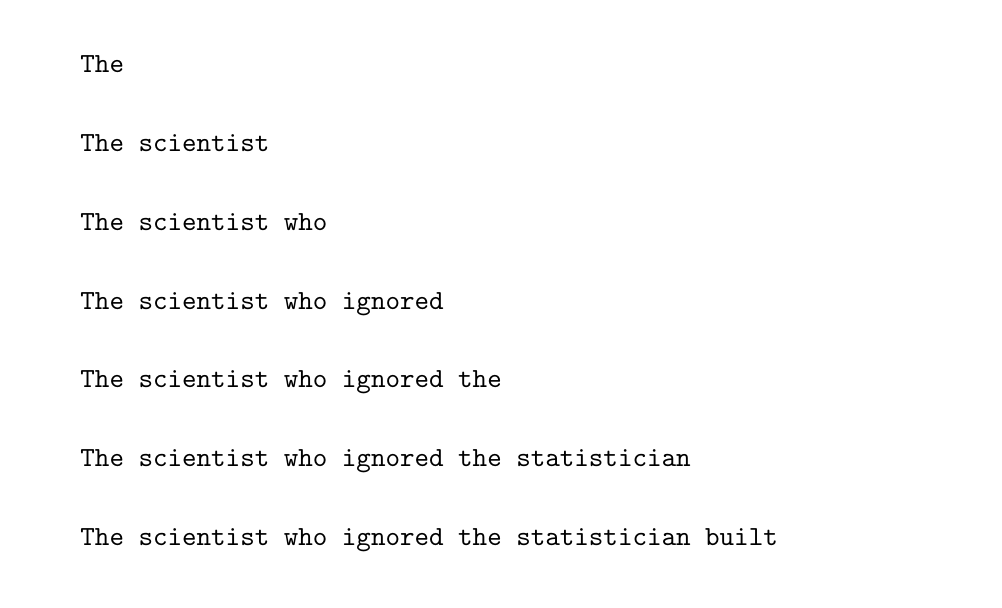
\begin{tikzpicture}[scale=1]

  \begin{scope}[shift={(0, 0)}]
    \draw[white] (-6, -0.5) rectangle (6, 0.5);
    \node[align=left] at (0, 0) { \texttt{The scientist who ignored the statistician built a model.} };
    \fill[white] (-4.75, -0.5) rectangle (6, 0.5);
  \end{scope}
  
  \begin{scope}[shift={(0, -1)}]
    \draw[white] (-6, -0.5) rectangle (6, 0.5);
    \node[align=left] at (0, 0) { \texttt{The scientist who ignored the statistician built a model.} };
    \fill[white] (-2.75, -0.5) rectangle (6, 0.5);
  \end{scope}
  
  \begin{scope}[shift={(0, -2)}]
    \draw[white] (-6, -0.5) rectangle (6, 0.5);
    \node[align=left] at (0, 0) { \texttt{The scientist who ignored the statistician built a model.} };
    \fill[white] (-2, -0.5) rectangle (6, 0.5);
  \end{scope}
  
  \begin{scope}[shift={(0, -3)}]
    \draw[white] (-6, -0.5) rectangle (6, 0.5);
    \node[align=left] at (0, 0) { \texttt{The scientist who ignored the statistician built a model.} };
    \fill[white] (-0.6, -0.5) rectangle (6, 0.5);
  \end{scope}
  
  \begin{scope}[shift={(0, -4)}]
    \draw[white] (-6, -0.5) rectangle (6, 0.5);
    \node[align=left] at (0, 0) { \texttt{The scientist who ignored the statistician built a model.} };    
    \fill[white] (0.1, -0.5) rectangle (6, 0.5);
  \end{scope}
  
  \begin{scope}[shift={(0, -5)}]
    \draw[white] (-6, -0.5) rectangle (6, 0.5);
    \node[align=left] at (0, 0) { \texttt{The scientist who ignored the statistician built a model.} };    
    \fill[white] (2.5, -0.5) rectangle (6, 0.5);
  \end{scope}
  
  \begin{scope}[shift={(0, -6)}]
    \draw[white] (-6, -0.5) rectangle (6, 0.5);
    \node[align=left] at (0, 0) { \texttt{The scientist who ignored the statistician built a model.} };   
     \fill[white] (3.6, -0.5) rectangle (6, 0.5);
  \end{scope}  

\end{tikzpicture}

\end{document}  